\begin{tikzpicture}
\tikzset{
    overlay box/.style={fill=white,fill opacity=0.9}
}
\node[overlay,anchor=north west,inner sep=0mm] (base) at (0, 0) {
    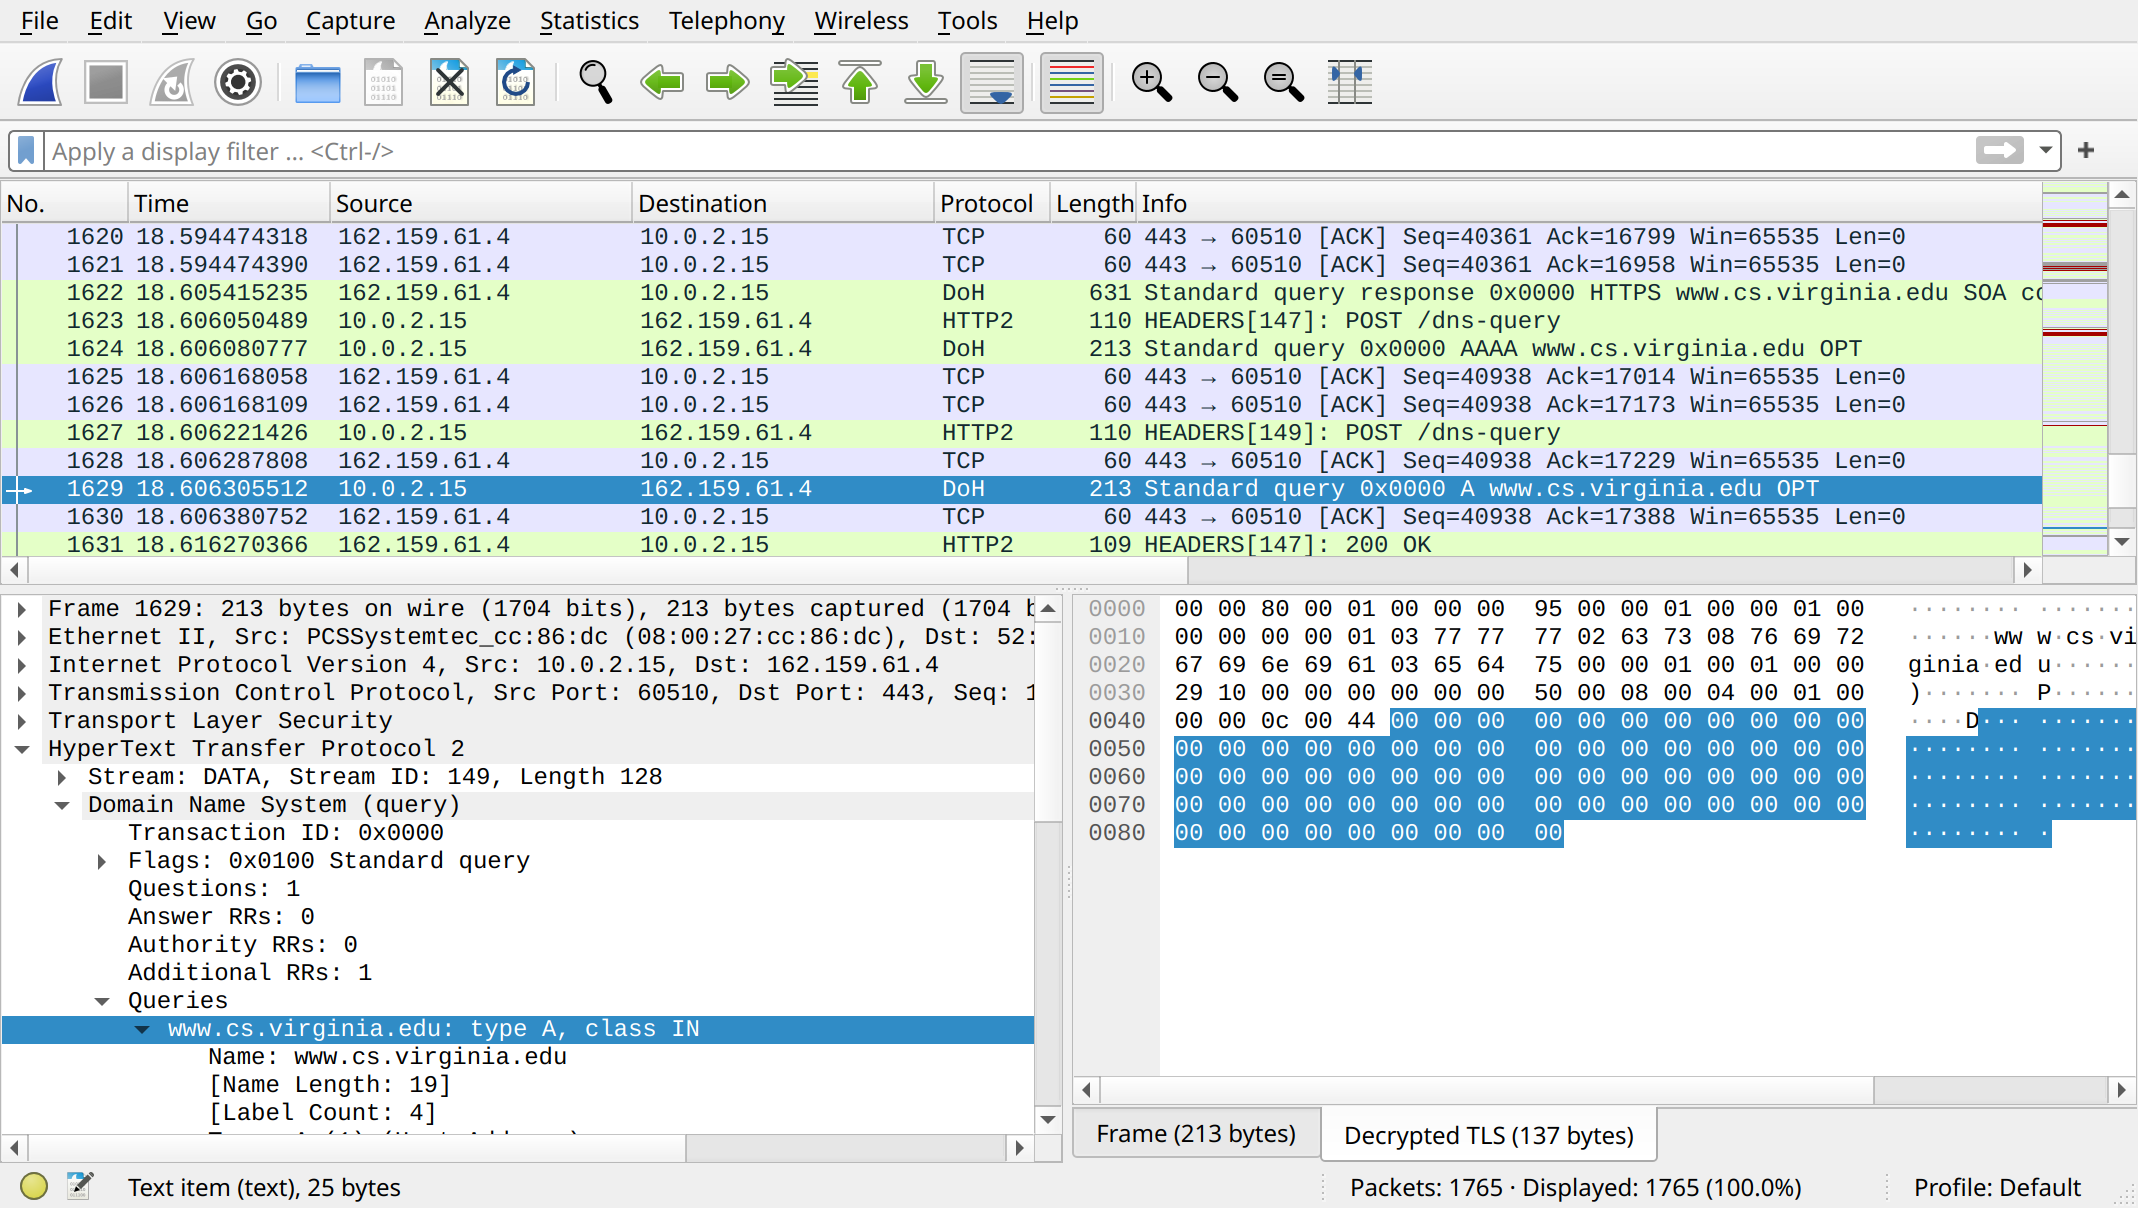
\includegraphics[width=\mypaperwidth]{../intro/wireshark-doh-zoom.png}
};
\path (0, 0) rectangle (14.5, -7); % for bounding box
%\draw[overlay,help lines] (0, 0) grid (14, -8);
    \begin{scope}
        \begin{pgfinterruptboundingbox}
    \tikzset{invclip/.style={clip,insert path={{[reset cm]
          (-16383.99999pt,-16383.99999pt) rectangle (16383.99999pt,16383.99999pt)
      }}}}
        \path[invclip] (6.3, -3.2) rectangle (7.15, -3.4);
        \end{pgfinterruptboundingbox}

        \fill[overlay,white,fill opacity=0.8] (0, 0) rectangle (14.5, -1.2);
        \fill[white,fill opacity=0.8] (0, -1.2) rectangle (14.5, -4);
        \fill[white,fill opacity=0.8] (7.25, -4) rectangle (14.5, -7.9);
    \end{scope}
    \path[draw,red,very thick] (0, -4) rectangle (7.25, -7.9);
    \tikzset{
        protomark/.style={Latex-,blue,thick},
        protomark alt/.style={Latex-,violet,thick,dotted},
        protomark brace/.style={blue,thick,decorate,decoration={brace}},
        protomark brace alt/.style={violet,thick,decorate,decoration={brace}},
        protomark label/.style={blue,fill=white,fill opacity=0.9},
    }
    \draw[protomark] (7.25, -4.3) -- ++(1, .2) node[right,protomark label] {ethernet};
    \draw[protomark] (7.25, -4.5) -- ++ (1, -.2) node[right, protomark label] {
                IPv4 (internet protocol version 4)
        };
    \draw[protomark] (7.25, -4.6) -- ++(1, -.6) node[right,protomark label] {
        TCP ({\fontsize{10}{11}\selectfont transmission control protocol})
    };
    \draw[protomark] (7.25, -4.8) -- ++(1, -1) node[right,protomark label] {
        TLS ({\fontsize{10}{11}\selectfont transport layer security})
    };
    \draw[protomark brace] (7.3, -5) -- (7.3, -7.9);
        \draw[protomark] (7.4, -6.5) -- ++ (0.75, 0) node[right, protomark label] {
            HTTP/2 ({\fontsize{10}{11}\selectfont hypertext transfer protocol 2})
        };
    \draw[protomark brace alt] (7.5, -5.5) -- (7.5, -7.9);
        \draw[protomark alt] (7.6, -6.85) -- ++ (0.75, -.5) node[right, protomark label] {
            DNS (domain name system)
        };
    \draw[red, very thick] (6.3, -3.2) rectangle (7.15, -3.4);
    \draw[red,Latex-,very thick] (7.15, -3.3) -- ++(1, 0) node[right,align=left,overlay box] {
        DoH = DNS over HTTPS
    };
\end{tikzpicture}